\chapter{The secrets of nature}
\label{chap:SM}

  This chapter attempts to understand the world around us using a mathematical framework which describes the matter and its interaction.
  Firstly, the laws that rule the Universe will be presented.
  Then, it will focus on the mathematical framework itself with the description of three interactions: the \gls{EM}, the weak and the strong interaction.
  Afterward, a framework that unifies the \gls{EM} and weak interaction, as well as the spontaneous symmetry breaking will be studied.
  Finally, the limits of this theory and the possible solution to overcome these issues will be tackled.
 
  \minitoc
  %\clearpage
  
  \section{The Standard Model}

    \subsection{Introduction}
     
    \begin{figure}[!h]
    \centering
      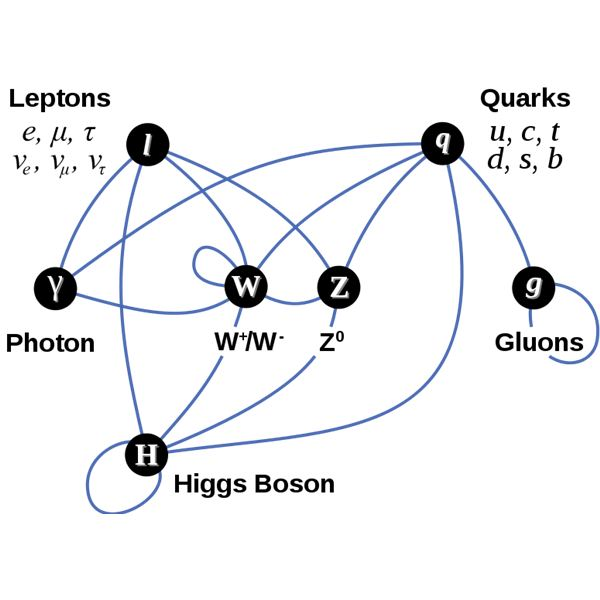
\includegraphics[width = 10cm]{Pictures/SM/elementaryParticles.jpg}
    %\missingfigure{Particles and boson}
    \caption{Summary of the Standard Model particles with their interactions \cite{SM}.}
    \label{fig:partInterac}
    \end{figure}   
    
    The \acrfull{SM} is a theory describing the elementary structure of the matter. 
    It is one of the most successful achievements in modern physics.
    The elegant theoretical framework of the \gls{SM} is explaining experimental results but predicts also a wide variety of phenomena.
    It depicts the interactions between the fundamental constituents of matter, called elementary particles.
    A quantum formalism describes an elementary particle with a set of quantum numbers.
    This quantum numbers are the spin, the intrinsic angular momentum, the parity P, the electric charge, etc.
    They are used to distinguish the 'matter' particles from the 'force carrier' particles.
    
    The half-integer spin particles obey to the Fermi-Dirac statistics and are submitted to the Pauli exclusion principle: they cannot occupy the same quantum state at the same time.
    These particles, that are the constituents of the matter, are called fermions and they are to the number of twelve types.
    The fermions are divided into two categories: the leptons and the quarks. 
    
    They are six lepton types: three charged particles and three neutral ones, called neutrino $\nu$.
    At the end of the $19^{\rm{th}}$ century, the first fundamental particles, the electron ($e^{-}$) was discovered by Thomson.
    The two other charged leptons were discovered in 1937 for the muon ($\mu$) and in 1975 for the tau ($\tau$).
    Three neutrinos are associated to the three flavored leptons: the electron neutrino ($\nu_e$) discovered in 1953, the muon neutrino ($\nu_{\mu}$) in 1962 \cite{Erwin1961} and the tau neutrino ($\nu_{\tau}$) discovered in 2000 \cite{DONUT2000}.

    The quarks are to the number of six.
    They cannot be found alone in nature.
    They are carrying a quantum number: the color.
    The color quantum numbers are green, blue and red (and the anti-color associated).
    They are always in a bounded state to form composite particles that are colorless and are called hadrons.
    A quark and an anti-quark form an integer spin composite particle, called a meson.
    Three quarks bounded together are called baryons. The most known baryons are the proton and the neutron.
    They are made of the up quarks ($u$) and the down quarks ($d$).
    The other quarks were discovered in the second half of the $20^{\rm{th}}$ century.
    The strange quark ($s$) was discovered in 1968, followed by the charm quark ($c$) in 1974.
    Then, the bottom quark or beauty quark ($b$) was discovered in 1977.
    The last quark discovered was the top quark ($t$) in 1995.  

    Depending on the particle's mass, the fermions are divided into three categories called generation.
    The first generation of particles forms the ordinary matter and is composed of the electron, the electron neutrino, the $u$ and $d$ quarks. 
    The two other generations are particles found in cosmic rays or in collisions with accelerators.
    All the fermions and their properties are summarised in table~\ref{tab:fermions}.

    \begin{table}[!h]
      \begin{center}
        \begin{tabular}{c c c c c c c}
        \hline %----------------------------
        Type & Family & Particle  & L & B & $\rm{Q}_e$ & Mass (MeV)  \tabularnewline
        \hline %----------------------------
        \hline %----------------------------
        \multirow{6}*{Leptons} & \multirow{2}*{1$^{st}$}    & $e$       & 1 & 0 & -1    & 0.511 \tabularnewline
                               & & $\nu_e$   & 1 & 0 & 0     & $< 2 \times 10^{-6}$ \tabularnewline
                               & \multirow{2}*{2$^{nd}$}    & $\mu$     & 1 & 0 & -1    & 105.66 \tabularnewline
                               & & $\nu_{\mu}$ & 1 & 0 & 0   & $< 2 \times 10^{-6}$ \tabularnewline
                               & \multirow{2}*{3$^{rd}$}    & $\tau$   & 1 & 0 & -1     & $1.78 \times 10^{3}$ \tabularnewline
                               & & $\nu_{\tau}$ & 1 & 0 & 0  & $< 2 \times 10^{-6}$ \tabularnewline
        \hline %----------------------------
        \hline %----------------------------
        \multirow{6}*{Quarks} & \multirow{2}*{1$^{st}$} & $u$ & 0 & 1 & 2/3 & $2.3^{+0.7}_{-0.5}$\tabularnewline
                              & & $d$ & 0 & 1 & -1/3 & $4.8^{+0.5}_{-0.3}$\tabularnewline
                              & \multirow{2}*{2$^{nd}$} & $s$ & 0 & 1 & -1/3 & $ 95\pm 5 $ \tabularnewline
                              & & $c$ & 0 & 1 &  2/3 & $1.275 \times 10^{3} \pm 2.5$ \tabularnewline
                              &\multirow{2}*{3$^{rd}$} & $b$ & 0 & 1 & -1/3 & $4.66 \times 10^{3} \pm 30 $ \tabularnewline
                              & & $t$ & 0 & 1 & 2/3 & $ 173.21 \times 10^{3} \pm 511 \pm 711$\tabularnewline
        \hline %----------------------------        
        \end{tabular}
      \end{center}
        \caption{Summary of the 12 types fermions. L is a quantum number associated to the leptons. Its value is 1 for leptons and -1 for anti-leptons. B is a quantum number associated to the baryons. It is equal to 1 for a baryon and to -1 for an anti-baryon \cite{Agashe:2014kda}. }
        \label{tab:fermions}
    \end{table}

    There is a second type of particles called bosons or gauge bosons.
    They have an integer spin and are following the Bose-Einstein statistics.
    Contrary to the fermions, the bosons are not limited to a single state occupancy.
    The bosons are the mediators of the four fundamental interactions, which are the followings:
    
    \begin{description}
      \item[\gls{EM} interaction:] It describes the interaction between two charges particles. 
      It is mediated by the photon $\gamma$, a massless and chargeless spin 1 particle.

      \item[Weak interaction:] It is the interaction responsible for the $\beta$ radioactive decay (a nucleon decays into another one with the emission of a lepton and a neutrino).
       The mediators of the weak interaction are the neutral electrical charged boson ($Z^0$) and two electrical charged bosons ($W^+$ and $W^-$).

      \item[Strong interaction:] It is responsible for the cohesion of the atom's nucleus, as well as the hadrons' cohesion.
      There are eight mediators called gluons.

      \item[Gravitational interactional:] It is not described by the \gls{SM}, but a quantum theory intends to associate a spin 2 boson, called graviton to the gravitational force.
      Nevertheless, finding a framework describing the equation of the general relativity and the equation of the quantum numbers is a difficult challenge.
    \end{description}

    %The interaction between two charges particles are mediated by the photon $\gamma$, a massless and chargeless spin 1 particle.
    %This interaction is called \gls{EM}.
    %The \gls{EM} is mediated by the photon $\gamma$, a massless and chargeless particle of spin 1.
    %The \gls{EM} is responsible for the interaction between two charged particles.
    %The weak interaction is responsible for the $\beta$ radioactive decay (a nucleon decays into another one with the emission of a lepton and a neutrino).
    %The mediators of the weak interaction are the neutral electrical charged boson $Z^0$, and two electrical charged gauge bosons: the $W^+$ and $W^-$.
    %The strong interaction is mediated by eight gauge bosons: the gluons.
    %The cohesion of the hadrons and the cohesion of the atom's nucleus is lead by the strong interaction.
    %The last force is the gravitational interaction but it is not included into the \gls{SM}.
    %Trying to find a framework where the equation of the general relativity used to describe the macroscopic world and the equation of the quantum mechanics describing the microscopic world is a difficult challenge.
    %A quantum theory intends to associate a boson to the gravitational force. 
    %This boson is a spin 2 particle and is called graviton.

    Another boson is predicted by the \gls{SM} but is not associated to a fundamental interaction, rather to the mass generation mechanism.
    It is the Higgs boson ($H$) that has been discovered in 2012 at the \gls{LHC} \cite{Aad2012}\cite{Chatrchyan2012}.
    The mass generation mechanism of particles is presented in section~\ref{sec:higgsMechanism}.
    

  \begin{table}[b]
    \begin{center}
        \begin{tabular}{c c c c c}
        \hline %----------------------------
        Force & Gauge bosons & Mass ($\rm{GeV/c}^2$) & Electric charge & Range \tabularnewline
        \hline %----------------------------
        \hline %----------------------------
        Electromagnetic & $\gamma$ & $0$ & $0$ & $\infty$\tabularnewline  
        \hline %----------------------------
        \multirow{2}*{Weak} & $Z^0$ & $91.1876 \pm 0.0021$ & $0$ & \multirow{2}*{$10^{-18}~\rm{m}$} \tabularnewline
             & $W^{\pm}$ & $80.3980 \pm 0.0250$ & $\pm 1$  &\tabularnewline 
        \hline %----------------------------
        Strong & g (8 gluons) & $0$ & $0$ & $10^{-15}~\rm{m}$ \tabularnewline
        \hline %----------------------------
        \hline %----------------------------
            & $H$ & $125~\rm{GeV}$ & $0$ & \tabularnewline
        \hline %----------------------------
        \end{tabular}
    \end{center}
    \caption{Summary of the interactions and the bosons defined in the Standard Model \cite{Agashe:2014kda}. The range corresponds to the distance on which the interaction is still effective. As the gravitational interaction is not part of the SM, the graviton is not included in this table.}
    \label{tab:bosons}
  \end{table}
    
    Table~\ref{tab:bosons} summarises the different bosons of the \gls{SM}.

    \subsection{Quantum Field Theory}

    The \gls{SM} is based on a mathematical framework called \gls{QFT}.
    It is a gauge theory, in which a Lagrangian describes an interaction following a particular symmetry.
    A symmetry is a transformation applied to a system that leaves it invariant.
    In 1918, Emmy Noether has demonstrated that all continuous symmetries of a system implies the conservation of a quantity during its evolution \cite{Noether1918}.
    For examples, symmetries under space translation and time translation imply respectively conversation of linear momentum and conversation of energy.

    In \gls{QFT}, the interactions are described by following gauge group:
    
      \begin{equation}
        \rm{SU}_{\rm{C}}(3) \otimes \rm{SU}_{\rm{L}}(2) \otimes \rm{U}_{\rm{Y}}(1),
      \end{equation}
    with $\rm{SU}_{\rm{L}}(2) \otimes \rm{U}_{\rm{Y}}(1)$ the symmetry group of the \gls{EW} interaction. 
    The subscript $L$ means that only the left-handed particles are interacting in the weak interaction, whereas the subscript $Y$ is associated to the hypercharge.
    The gauge symmetry group associated to the strong interaction is $\rm{SU}_{\rm{C}}(3)$.
    The subscript $C$ means that only the particles that have a color charge are interacting via the strong interaction.

    The gauge theory is invariant under a continuous set of local transformations.
    Taking the gauge symmetries and the least action into account, physicists were able to set up equations that describe the dynamic of the interactions by a Lagrangian.
    The steps to build Lagrangian for the three forces and the unification of the \gls{EM} and weak interactions are going to be presented. 

      \subsubsection{Quantum Electrodynamic}
      
      \gls{QED} is the \gls{QFT} that combines the electromagnetism and the quantum mechanics formalisms.
      The interactions are described using a relativistic Lagrangian that is invariant under a continuous set of transformation.
      For a free fermion with a mass $m$, the Dirac Lagrangian $\mathcal{L}_{\rm{Dirac}}$ is:

      \begin{equation}
        \mathcal{L}_{\rm{Dirac}} = \overline{\Psi}\left(x\right) \left(i \gamma^{\mu}\partial_{\mu} - m \right) \Psi\left(x\right),
        \label{eq:diracLag}
      \end{equation}
      with $\Psi\left(x\right)$ the spinor field describing the fermion and $\gamma^{\mu}$ are the Dirac matrices. 
      
      As \gls{QED} is built on a local gauge symmetry, the Lagrangian must be invariant under global $\rm{U}(1)$ transformations:
      
      \begin{equation}
            \begin{array}{rrccr}
             \Psi \left(x \right) & \rightarrow & \Psi^{'} \left(x \right)  & = & e^{-i\alpha} \Psi\left(x\right), \\
             \overline{\Psi}\left(x\right) & \rightarrow & \overline{\Psi}^{'}\left(x\right) & = & e^{i\alpha}  \overline{\Psi}\left(x\right). \\
            \end{array}
        \label{eq:globalTransformations}
      \end{equation}

      The corresponding local symmetry is:

      \begin{equation}
            \begin{array}{rcccr}
             \Psi\left(x\right) & \rightarrow & \Psi^{'} \left(x \right) & = & e^{-i\alpha(x)} \Psi\left(x\right), \\
             \overline{\Psi}\left(x\right) & \rightarrow & \overline{\Psi}^{'}\left(x\right) & = & e^{i\alpha(x)}  \overline{\Psi}\left(x\right). \\
            \end{array}
        \label{eq:localTransformations}
      \end{equation}

      By applying the transformation of equation~\ref{eq:globalTransformations}, the Lagrangian from equation~\ref{eq:diracLag} becomes:

      \begin{equation}
        \mathcal{L}^{'}_{\rm{Dirac}} = \mathcal{L}_{\rm{Dirac}} - \overline{\Psi} \gamma^{\mu} \Psi \partial_{\mu} \alpha.
        \label{eq:diracLag2}
      \end{equation}
      
      Although the mass term of the Lagrangian in equation~\ref{eq:diracLag2} stays invariant under the local symmetry, the term containing a partial derivative does not.
      To keep the Lagrangian invariant, a gauge field $A_{\mu}$ is introduced:

      \begin{equation}
        A_{\mu} \rightarrow A_{\mu} - \frac{1}{e} \partial_{\mu} \alpha.
      \end{equation}

      Moreover, the partial derivative is replaced by a covariant one:

      \begin{equation}
        D_{\mu} \Psi\left(x\right) =  \left(\partial_{\mu} - i Q_e A_{\mu}\right) \Psi\left(x\right).
      \end{equation}

      The gauge field is not yet a dynamic field. 
      To get a physical gauge field, a kinetic term should be added to the equation.
      This gauge invariant term that includes derivative from the $A_{\mu}$ field is:
    
      \begin{equation}
        F_{\mu \nu} \ = \ \partial_\mu A_\nu - \partial_\nu A_\mu.
      \end{equation}

      The Lagrangian, which is local invariant, is the one that describes the \gls{QED}:

      \begin{equation}
          \mathcal{L}_{\rm{QED}} =  \overline{\Psi}\left(x\right)\left( i \gamma^\mu D_\mu - m \right) \Psi\left(x\right) - \frac{1}{4}F_{\mu \nu}\left(x\right) F^{\mu \nu}\left(x\right).
      \end{equation}

      A mass term $m A_{\mu} A^{\mu}$ for the field $A_{\mu}$ is missing because it would break the gauge invariance.
      That consideration matches to the fact that the photon is a massless boson.

    \todo{Add details on the QED: coupling...}

    \subsubsection{Weak interaction}

    In 1930, Pauli has explained the continuous spectrum of the electron in the $\beta$ decay by the existence of new particle which respects the principle of energy conservation.
    It is a light particle, which does not interact so much with matter.

    After the discovery of the neutron by Chadwick in 1932 \cite{chadwick1932possible}, Fermi wrote a theory on weak interaction to explain the $\beta$ decay \cite{Fermi:1934hr}. 
    He postulated that the neutron is decaying into a proton by emitting an electron and a light neutral particle, called neutrino.
    In analogy to the electromagnetism, he proposed a current-current Lagrangian to describe the $\beta$ decay.
    \begin{equation}
      \mathcal{L}_{\rm{weak}} = \frac{G_F}{\sqrt{2}}\left(\overline{p} \gamma_{\mu} n \right) \left(\overline{e} \gamma_{\mu} \nu \right),
    \end{equation}
    where, $G_F$ is the Fermi constant $G_F = 1.166 \cdot 10^{-5}~\rm{GeV}^{-2}$. $p$, $n$, $e$ and $\nu$ are respectively the vector currents describing the proton, the neutron, the electron and the neutrino. 
    
    Nevertheless, the non-relativistic limit leads to an incomplete theory.
    The interaction considered with a 2-components spinor transforms a proton into a neutron without changing the position, the spin or the parity.
    However, Lee and Yang have postulated in 1956 that the weak interaction violates the parity after analysing the decays of the $\tau$ and $\theta$ particles \cite{1956PhRv..104..254L}.
    The Wu experiment \cite{1957PhRv..105.1413W} confirmed this hypothesis in 1957 by studying the decay of $^{60}$Co.

    The Fermi interaction was modified by Feynman and Gell-Mann \cite{PhysRev.109.193} to a $V~-~A$ theory\footnote{$V$ stands for vector and $A$ for axial-vector}.
    The vector current is now subtracted by an axial vector current. 
    For example, the neutrino current is replaced by:

    \begin{equation}
        \begin{array}{rcc}
        \overline{e}(x) \gamma_{\mu} \nu & \rightarrow & \overline{e}\gamma_{\mu}(1 - \gamma_5 ) \nu \\
            & & = \overline{e} \gamma_{\mu} \nu - \overline{e}\gamma_{\mu} \gamma_5 \nu, \\
        \end{array}
    \end{equation}
    with $\overline{e} \gamma_{\mu} \nu$ a current vector and $\overline{e}\gamma_{\mu} \gamma_5 \nu$ an axial current vector.

    It was established that the weak current has the form $V~-~A$ instead of $V~+~A$.
    The weak interaction is only coupling left-handed particles and right-handed anti-particles.
    The Lagrangian describing the weak interaction can be written as a current interaction:

    \begin{equation}
      \mathcal{L}_{\rm{weak}} = - \frac{G_F}{\sqrt{2}} J^{\mu}J_{\mu}^{\dagger},
    \end{equation}
     and $J^{\mu}$ is a combination of leptonic and hadronic currents.

    Contrary to \gls{QED}, the weak interaction obeys to a non-Abelian symmetry group\footnote{A group is non-Abelian when the elements of the group are not commutating.}, the $\rm{SU}(2)$ symmetry group.
    The matter field could be represented as a doublet $\Psi_L$ and a singlet $\Psi_R$ of this group.

    \begin{equation}
      \begin{array}{cc}
        \Psi_L = 
         \begin{pmatrix}
           \nu_{eL} \\
           e_L
         \end{pmatrix}, & \Psi_R = e_R.
      \end{array}
    \end{equation}

    The generators of the group are the three Pauli matrices $\sigma_i$, associated with a gauge field $W_{\mu}^i$.
    The bosons of the weak interactions are the $W^{\pm}$ and $Z$.

    As the left-handed leptons are combined into a doublet, a quantum number called weak isospin ($I_3$) is associated with them.
    The charged leptons have a weak isospin $I_3 = -\frac{1}{2}$ and for the neutrinos $I_3 = \frac{1}{2}$.
    Concerning the gauge bosons $W^{\pm}$ and $Z$, the weak isospin is respectively $I_3 = \pm 1, 0$.
    
    \subsubsection{Quantum Chromodynamics}
    
    \gls{QCD} is the quantum field theory of the strong interaction.
    In this model, the interaction is due to an $\rm{SU}(3)$ gauge group. 
    It produces 8 gauge fields called gluons.
    The spinors of this theory are the six quarks that form a triplet with respect to the gauge symmetry.

    The $\rm{SU}(3)$ gauge group is a group of $9 - 1 = 8$ real parameters and of 8 generators. 
    Those generators are the Gell-Mann matrices. 
    The normalised generators are defined by: 
    
    \begin{equation}
        T^a = \frac{1}{2}\lambda^a.
    \end{equation}

    The structure constant $f^{abc}$ can be expressed as:

    \begin{equation}
        if^{abc} = 2 Tr([T^a,T^b]T^c).
    \end{equation}
     
    Each of them is considered as a triplet state with respect to the $\rm{SU}(3)$ group:

    \begin{equation}
      q_i = 
        \begin{pmatrix}
          q_i^1 \\
          q_i^2 \\
          q_i^3 \\
        \end{pmatrix},
     \end{equation}
    where $q_i$ are the six quarks, that can have three different states, called color.
    These charged colors are red, blue and green.

    As the local gauge symmetry $\rm{U}(1)$ is included into the $\rm{SU}(3)$ group, the gauge field $A_{\mu}$ is modified to be:
    
    \begin{equation}
      A_{\mu} = g_S A^a_{\mu}\frac{\lambda^a}{2},
    \end{equation}
    with $a = 1,\cdots,8$ and corresponds to the 8 gluons.
    To keep the gauge invariance, there is no mass term $m_g A^{\mu}_a A^a_{\mu}$.
    Then, the gluons are massless. 

    The covariant derivative is also rewritten to keep the gauge invariance:

    \begin{equation}
      \begin{array}{rcl}
        D_{\mu} & = & \partial_{\mu} - i A_{\mu} \\
                & = & \partial_{\mu} - i g_S A^a_{\mu} \frac{\lambda^a}{2}.
      \end{array}
    \end{equation}

    The \gls{QED} field $F_{\mu \nu}$ is not gauge invariant in \gls{QCD}.
    Nevertheless, an additional term to obtain gauge invariant field tensor can be introduced:
    
    \begin{equation}
      G^a_{\mu \nu} = \left( \partial_{\mu} A^a_{\nu} - \partial_{\nu} A^a_{\mu} \right) + g_S f^{abc} A^b_{\mu} A^c_{\nu}.
    \end{equation} 

    Finally, the \gls{QCD} Lagrangian is given by:

    \begin{equation}
      \mathcal{L} = \sum_{i=1}^6  \bar{q_i} \left(i \gamma^{\mu}D_{\mu} -m_i \right)q_i - \frac{1}{4} G_{\mu \nu}^{a} G_{a}^{\mu \nu}.
    \end{equation}
    
    %\section{The Glashow-Weinberg-Salam model}
    \section{Towards a unified theory}

    Late 1960, a model of unification was postulated by Glashow, Weinberg, and Salam to describe the \acrfull{EW}.
    The theory rests on a  $\rm{SU}(2)_{\rm{L}} \otimes \rm{U}(1)_{\rm{Y}}$ symmetry group.
    It is the simplest group which conserves the properties of EM charge conversion and parity violation of weak interaction.

    For the~\gls{EW} unification, the $\rm{U}(1)_{\rm{EM}}$ symmetry group describing  the \gls{EM} interaction has to be rewritten.
    As the fermions are considered by left-handed doublets and right-handed singlets, the $\rm{U}(1)_{\rm{EM}}$ breaks the gauge invariance.
    The weak isospin group $\rm{SU}(2)_{\rm{L}}$ is combined with the EM charge to create the hypercharge give by the Gell-Mann-Nishijima relation: 
  
    \begin{equation}
      Q = I_3 + \frac{1}{2}Y.
    \end{equation}
   
    The $I_3$ term is the third component of the weak isospin.
    With the introduction of the hypercharge, the EM gauge invariance is conserved.

    The \gls{EW} Lagrangian is:

    \begin{equation}
      \mathcal{L}_{\rm{EW}} = \mathcal{L}_{\rm{YM}} + \mathcal{L}_{\rm{fermions}}.
      \label{eq:ewLag}
    \end{equation}

    The first term $\mathcal{L}_{\rm{YM}}$ is the Yang-Mills Lagrangian that describes the bosons gauges interactions (kinetic term + interaction between bosons). 
    It has the form below:

    \begin{equation}
      \mathcal{L}_{\rm{YM}} = - \frac{1}{4}\textbf{W}^a_{\mu\nu} \textbf{W}^{a\mu\nu} - \frac{1}{4}\textbf{B}_{\mu\nu}\textbf{B}^{\mu\nu},
    \end{equation}
    where $\textbf{W}^{a}_{\mu\nu}$ ($i=1,2,3$) and $\textbf{B}_{\mu\nu}$ are the gauge fields corresponding respectively to $\rm{SU}(2)$ and $\rm{U}(1)$ groups.
    The tensors of these fields are written:

    \begin{equation}
        \textbf{W}_{\mu\nu}  =  \partial_{\mu}\textbf{W}_{\nu} - \partial_{\nu}\textbf{W}_{\mu} - i g [\textbf{W}_{\mu},\textbf{W}_{\nu}]~\rm{and}
      \label{eq:Wmunu}
    \end{equation}

    \begin{equation}
        \textbf{B}_{\mu\nu}  =  \partial_{\mu}\textbf{B}_{\nu} - \partial_{\nu}\textbf{B}_{\mu}.
        \label{eq:Bmu}
    \end{equation}
   
    Where $g$ is the coupling constant of the $\rm{SU}(2)$ gauge group. 
    In equation~\ref{eq:Wmunu}, $\textbf{W}_{\mu} = \sum W^i_{\mu}\sigma^i/2$ is a vector of three gauge fields associated to $\rm{SU}(2)_{\rm{L}}$ and $\sigma^i$ are the Pauli matrices. 
    The term $[\textbf{W}_{\mu},\textbf{W}_{\nu}]$ is associated to the interactions between the gauge fields.
    In equation~\ref{eq:Bmu}, $\textbf{B}_{\mu}$ is the only gauge field associated to the $\rm{U}(1)_{\rm{Y}}$ gauge group.

    The Lagrangian describing the fermions field is given by:

    \begin{equation}
      \mathcal{L}_{\rm{fermions}} = \overline{\Psi}_L\gamma^{\mu}D_{\mu}\Psi_L + \overline{\Psi}_R\gamma^{\mu}D_{\mu}\Psi_R,
    \end{equation}
    with:
      
    \begin{equation}
      \begin{array}{lcl}
      D_{\mu}\Psi_L & = & \left( \partial_{\mu} + ig \textbf{W}_{\mu} - i \frac{g'}{2} Y \textbf{B}_{\mu}\right)\Psi_L~\rm{and} \\
      D_{\mu}\Psi_R & = & \left(\partial_{\mu} - i\frac{g'}{2} Y \textbf{B}_{\mu}\right)\Psi_R.
      \end{array}
      \label{eq:derivativeEW}
    \end{equation}
    
    In equation~\ref{eq:derivativeEW}, the covariant derivative has two forms. 
    The weak interaction does not allow coupling of the $W$ bosons to right-handed fermions, whereas the $\gamma$ and $Z$ bosons do.

    With the \gls{EW} Lagrangian described above, the gauge bosons are considered as massless fields.
    The electroweak interaction does not allow a $m\overline{\Psi}\Psi$ term because it does not transform as a scalar under $\rm{SU}(2)_{\rm{L}} \otimes \rm{U}(1)_{\rm{Y}}$.
    Moreover, the $m^2 \textbf{W}_{\mu} \textbf{W}^{\mu}$ violates the $\rm{SU}(2)_{\rm{L}}$ gauge invariance of the Lagrangian.
    The mass terms associated with the physical fields of the gauge bosons are given by a spontaneous symmetry breaking via the Higgs mechanism.

      \subsection{Symmetry Breaking mechanism and Goldston theorem}
    
      Before introducing the Higgs mechanism, the spontaneous symmetry breaking is presented for a global symmetry.
      This phenomenon appears in other physics fields, such as the phase transition or laser theory.

      A Lagrangian density for a complex scalar field $\phi$ is considered here:

      \begin{equation}
        \mathcal{L} = \partial^{\mu}\phi^{*} \partial_{\mu}\phi - \mu^2\phi^{*}\phi - \lambda (\phi^{*}\phi)^2,
        \label{eq:ssbLagrangian}
      \end{equation}
      where $\partial^{\mu}\phi^{*} \partial_{\mu}\phi$ is the kinetic term of a complex scalar field and $\mu^2\phi^{*}\phi - \lambda (\phi^{*}\phi)^2$ is related to a scalar potential.
      The coefficient $\mu^2$ is a real parameter. 
      Nevertheless, depending on its sign, the potential can take two forms.

      If $\mu^{2} > 0$, the symmetry is unbroken and the potential has a minimum at $\phi = 0$ which does not degenerate.
      It describes a particle with a mass $\mu$ and a quartic self-coupling.
      As the transformation $\phi \rightarrow  - \phi$ is respected, this solution is a symmetric one.

      When $\mu^{2} < 0$, there is not a unique ground state for this system but multiple states with the same vacuum energy.
      The minima is located on a circle of radius:

      \begin{equation}
        v = \sqrt{\frac{- \mu^2}{2\lambda}} > 0.
        \label{eq:v}
      \end{equation}

      By choosing a particular solution as the ground state, the symmetry gets spontaneously broken.
      A parametrisation of the excitations around the ground state is possible by introducing a new field $\phi$:

      \begin{equation}
        \phi(x) = \frac{1}{\sqrt{2}} \left( v + \rho(x) + i\Theta(x) \right),
      \end{equation}
      with $\rho(x)$ and $\Theta(x)$ real fields and the value $v$ is given by one of the solution from equation~\ref{eq:v}.
      By injecting this new field in equation~\ref{eq:ssbLagrangian}, the Lagrangian becomes:

      \begin{equation}
        \mathcal{L} = \frac{1}{2} (\partial_{\mu}\rho)^2 + \frac{1}{2}(\partial_{\mu}\Theta)^2 - \lambda v^2 \rho^2 - \lambda v (\rho^3 +\rho \Theta^2) - \frac{\lambda}{4}(\rho^2 + \Theta^2)^2,
      \end{equation}
      where the field $\rho(x)$ describes a state of mass $m_{\rho} = 2 \mu^2$, coupled to the massless field $\Theta(x)$.
      The field $\Theta(x)$ describes excitations around a direction in the potential.
      These excitations are not costing any energy to the system and they correspond to massless bosons called Goldstone bosons.

      \subsection{Higgs mechanism}
      \label{sec:higgsMechanism}
      
      As seen with the \gls{QED} and \gls{QCD} Lagrangian, the bosons generated are massless.
      Nevertheless, the $W^{\pm}$ and $Z$ bosons have a mass and equation~\ref{eq:ewLag} of \gls{EW} interaction does not include a mass generator.
      The Higgs-Englert-Brout mechanism solves the origin of the fermions masses \cite{PhysRevLett.13.508}\cite{1964PhRvL..13..321E}.
       
      The invariant Lagrangian density under $\rm{SU}(2)_{\rm{L}} \otimes \rm{U}(1)_{\rm{Y}}$ gauge transformation is:

      \begin{equation}
        \mathcal{L} = \left(D^{\mu} \Phi \right)^{\dagger} \left( D_{\mu} \Phi \right) - V(\Phi),
        \label{eq:lagrangianHiggs}
      \end{equation}    
      with $\Phi$ a doublet of complex scalar fields defined as following:
      
      \begin{equation}
         \Phi = \begin{pmatrix}
                  \phi^{+}\\
                  \phi^{0}
                \end{pmatrix}.
      \end{equation}

      The covariant derivative in equation~\ref{eq:lagrangianHiggs} is the one of $\rm{SU}(2)_{\rm{L}} \otimes \rm{U}(1)_{\rm{Y}}$ given by equation~\ref{eq:derivativeEW} and represents the kinetic term.
      The Higgs potential is similar to the one considered first and has also two solutions depending on the sign of $\mu^2$, but only the negative solution is shown here.
      There is an infinite set of degenerated states with minimum energy:

      \begin{equation}
        \phi_0 = \sqrt{\frac{1}{2}}
        \begin{pmatrix}
          0 \\
          v
        \end{pmatrix}
        ~\rm{with}~v = \sqrt{\frac{- \mu^2}{\lambda}} > 0.
        \label{eq:v2}
      \end{equation}
      
      The field $\Phi$ is expanding around its minima using a new field $h(x)$, which describes quantum fluctuations.
      Moreover, three massless Goldstone fields $\theta^{i}(x)$ are included:

      \begin{equation}
        \Phi(x) = e^{i\frac{\sigma_i}{2}\theta^i(x)} \frac{1}{\sqrt{2}}
                  \begin{pmatrix}
                     0 \\
                     v + h(x)
                   \end{pmatrix}.
        \label{eq:fieldHiggs}
      \end{equation}
       
      By choosing a particular gauge field, the Goldstone fields are absorbed into the physical field defined by $\rm{SU}(2)_{\rm{L}} \otimes \rm{U}(1)_{\rm{Y}}$.
      The absorption of the massless Goldstone bosons leads to the apparition of a mass term in equation~\ref{eq:lagrangianHiggs}.
      The mass generation mechanism is explained in the following.
      The new field injected in equation~\ref{eq:lagrangianHiggs} modifies the derivative covariant.
      By omitting any terms containing $h$ and by removing the partial derivative: 

      \begin{equation}
        \left|\left(i\frac{g}{2}\textbf{W}_{\mu} +i\frac{g'}{2}Y\textbf{B}_{\mu}\right) \Phi \right|^2 = \frac{1}{8}\left|
                \begin{pmatrix}
                   gW^3_{\mu} +g'B_{\mu} & g(W^1_{\mu} - i W^2_{\mu}) \\
                   g(W^1_{\mu} + i W^2_{\mu}) & - g W^3_{\mu} + g'B_{\mu}
                \end{pmatrix}
                \begin{pmatrix}
                  0 \\
                  v
                \end{pmatrix}
           \right|^2.
        \label{eq:derHiggs}
      \end{equation}

      The charged fields can be expressed as a linear combination of gauge fields:

      \begin{equation}
        W^{\pm}_{\mu} = \frac{W^1_{\mu} \mp iW^2_{\mu}}{\sqrt{2}}.
      \end{equation}

      The eigenstates are rewritten as decorrelated terms representing the neutral fields from the \gls{EW} symmetry group:

      \begin{equation}
        Z_{\mu} = \cos{\theta_{w}W^3_{\mu}} - \sin{\theta_{w}B_{\mu}},
      \end{equation}
      \begin{equation}
        A_{\mu} = \sin{\theta_{w}W^3_{\mu}} + \cos{\theta_{w}B_{\mu}},
      \end{equation}
      with $\theta_{w}$ the Weinberg angle, which represents a bound between the couplings $g$ and $g'$:
     
      \begin{equation}
        \sin{\theta_{w}} = \frac{g'}{\sqrt{g^2+g'^2}} \ and \ \cos{\theta_{w}} = \frac{g}{\sqrt{g^2+g'^2}}.
      \end{equation} 

      Equation~\ref{eq:derHiggs} becomes:

      \begin{equation}
        \begin{array}{rcl}
       \left|\left(i\frac{g}{2}\textbf{W}_{\mu} +i\frac{g'}{2}Y\textbf{B}_{\mu}\right) \Phi \right|^2 & = & \frac{1}{8} \left| 
          \begin{pmatrix}
            A_{\mu}\sqrt{g^2 + g'^2} & gW^-_{\mu} \\
            gW^+_{\mu} & -Z_{\mu}\sqrt{g^2 + g'^2}
          \end{pmatrix}
       \right|^2 \\
        & = & \frac{1}{2}M^2_Z ZZ^* + \frac{1}{2}M^2_W W^-W^+
        \end{array}
      \end{equation}

      With $M_Z = \frac{1}{2}v\sqrt{g^2 + g'^2}$ and $M_W = \frac{1}{2} vg$, the mass of the $Z$ boson and the W$^{\pm}$ bosons. 
      The mass of the photon is consistent with the expectation and is null. 

      The Higgs mechanism implies the existence of a massive gauge field, the Higgs boson.
      It is coupled to the other bosons and also to itself.
      This could be shown by extending the Higgs potential with the field defined in equation \ref{eq:fieldHiggs}:

      \begin{equation}
        -\lambda v^2h^2 - \lambda v h^3 - \frac{1}{4}\lambda h^4
      \end{equation}

      The first term gives the mass of the Higgs boson, $M^2_H = 2\lambda v^2$, while the second and third terms are the Higgs self-interactions.
      The Higgs mass can not be predicted by the theory because it is given by a function of the parameter $\lambda$, which is one of the free parameters of the \gls{SM}.
      
      \begin{figure}[h]
      \centering
        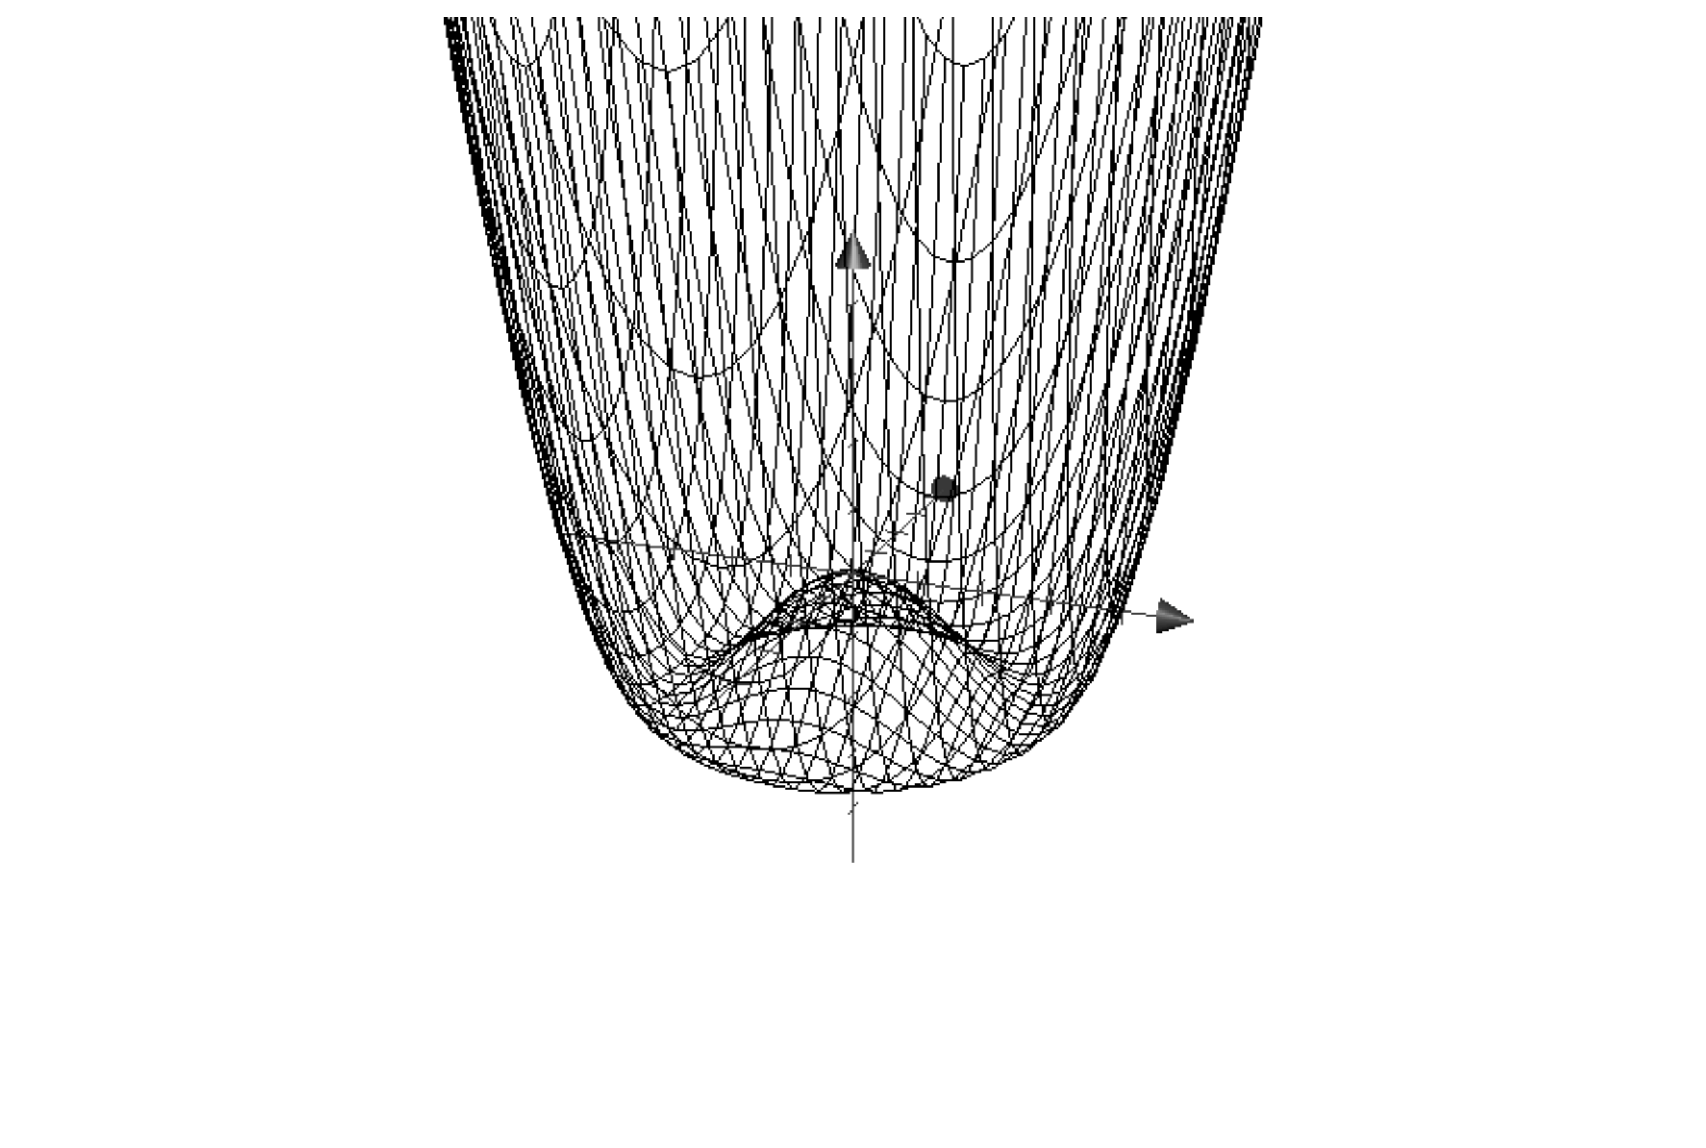
\includegraphics[width = 10cm]{Pictures/SM/mexHat.eps}
      \caption{Higgs potential $V(\phi)$ for $\mu^2 < 0$.}
      \label{fig:scalarPotential}
      \end{figure}

      \todo{Yukawa couplings with fermions}

  \section{Beyond the Standard Model}

  The \gls{SM} constitutes one of the most successful achievements in modern physics.
  One of its strength is to provide an elegant theoretical framework to describe the known experimental facts about particles, but it also predicts the existence of a mechanism to generate the particle masses via the Higgs mechanism.
  Nevertheless, this theory does not solved all the questions about the Universe.
  \todo{Add plots to confirm the good SM predictions.}
  
    \subsection{Limitations of the Standard Model}

    In the following, the limitations of the \gls{SM} are described.

    %Despite the fact that the experimental results are in good agreement with the \gls{SM} predictions, this theory does not provide answers to may questions.
    %The particle physics community tries to unify theories.

      \subsubsection{Free parameters}

      Up to 19 free parameters are used in the \gls{SM} and this theory does not explain their existence.
      Even if it is not as major problem for the physics itself, the particle physics community has a lack of understanding and explaining these values.
      These free parameters are: 
      \begin{itemize}
        \item the masses of the nine fermions,
        \item the coupling constants $g$ and $g'$ of respectively the $U(1)$ and $SU(2)$ groups,
        \item the coupling constant of the strong interaction $\alpha_s$,
        \item the three mixing angles, as well as the CP-violating phase of the CKM matrix,
        \item the Higgs boson mass and the expected vacuum value for the Higgs field $vev$,
        \item $\theta^{\rm{QCD}}_{\rm{CP}}$, a parameter that allows the CP violation in \gls{QCD}.
      \end{itemize}

      To this 19 free parameters, 7 other parameters can be considered, thus increasing the number of parameters to 26.
      This parameters are the masses of the three neutrinos, as well as the four parameters of the \textit{Pontecovro-Maki-Nakagawa-Sakata} matrix\footnote{equivalent of the CKM matrix for the neutrinos' mass}.
    
      \subsubsection{Hierarchy problem}


      The hierarchy problem refers to two main energy scales problem of the \gls{SM}.
      First of all, the difference between the energy scale of the \gls{SM} and the Planck scale is of seventeen orders of magnitude.
      No "intermediate" physics has been found between the two scales.
      A second problem occurs while considering the Higgs boson mass.
      The \gls{SM} does not predict its mass, but it sets some theoretical bounds with respect to $\Lambda$, the energy scale at which the \gls{SM} is not valid anymore.
      The theoretical Higgs boson mass is higher than what it should be compared to the EW scale.
      The Higgs boson interacts with the particles of the \gls{SM} (fermions, $W$ and $Z$ boson), but it also interacts with itself.
      Due to the scalar nature of the boson, there are quartic divergences while calculating the loop corrections.
      The quantum corrections, which take into account the coupling of the Higgs boson, are $\Lambda^2$ divergent and lead to a huge Higgs boson mass.
      To avoid that, delicate cancellations should occur between the quantum corrections.
      These cancellations are known as the fine-tuning problem. 
      
      \subsubsection{Gravitation}

      Although particle physicists are dreaming of a "theory of everything" that will unify the electroweak, strong and gravitational interactions, there is no viable theory to describe the gravity in a quantum point of view to include it in the \gls{SM} and which would be still valid at a macroscopic scale.

      \subsubsection{Neutrino mass}

      The neutrinos defined by the \gls{SM} are assumed to be exactly massless.
      Nevertheless at the end of the year 1990, the Super Kamiokande experiment had surprising results \cite{Super-Kamiokande-Oscillation}.
      The measured flux of solar and atmosphere neutrons was lower than expected.
      The result was interpreted by an oscillation of neutrinos between the three leptonic flavors.
      However, the oscillation is possible only if the neutrino has a mass and if the leptonic number is violated \cite{Dib}.
      That phenomenon could be considered as a proof of physics beyond the \gls{SM}.

      \subsubsection{Matter-antimatter asymmetry}

      As discussed at the beginning of this chapter, the \gls{SM} defines an equal number types of particles and anti-particles. 
      In the case of the Big Bang theory, it is assumed that the matter and antimatter were created in an exactly equal amount.
      However, if the amount of matter and antimatter was equal, the Universe would have been completely annihilated.
      A mechanism has favoured electrons, protons and neutrons with respect to positrons, antiprotrons and antineutrons.
      The asymmetry between the matter and antimatter proportion could come from a smaller production of antimatter compared to the matter during the Big Bang.
      The matter and antimatter have annihilated, but a part of matter has survived. 

      The study of the kaon oscillation has shown that this particle is able to transform spontaneously to its own antiparticle and vice-versa.
      Nevertheless, this transformation is not symmetric: the kaon is slower to turn into an anti-kaon than the inverse transformation.

      \subsubsection{Dark Matter and dark energy}
      
     % \todo{Rephrase dark matter and dark energy}
      Several astrophysical observations are indicating that the Universe is made not only of visible matter but also of matter that seems to be invisible to the electromagnetic interaction and is called the dark matter.
      In 1933, a measurement of the galaxies velocities in the Coma cluster to determine the cluster mass gives a surprising result.
      The mass was more than two orders of magnitude bigger than the mass of visible stars in the cluster.
      It was found that the matter of the \gls{SM} describes only $5~\%$ of the Universe content. 
      The rest of the Universe is made of $22~\%$ of dark matter and around $73~\%$ of dark energy.
      The neutrinos are possible candidates to dark matter, as they couple to \gls{SM} matter only via weak interaction, but they cannot account for the entire density of the universe.
      Nowadays only twelve particles (plus the anti-particles associated) have been observed. 

    \subsection{Theories beyond the Standard Model}

      Several theories try to complete the \gls{SM}. 
      They do not try to solve completely all the problem enumerated above, but they focus on either a specific problem, either on adding new degrees of freedom.
      This section presents the different problems that can be solved with these theories beyond the \gls{SM}.

      \subsubsection{Supersymmetry}
    
      The \gls{SUSY} is a \gls{QFT}, that relates the elementary fermions known to corresponding new bosons, called sfermions and the bosons to corresponding new fermions, called sbosons \cite{Signer2009}.
      The new particles introduced are called super-partners.
      Table~\ref{tab:SUSY} summarises the super-partners associated to the \gls{SM} particles for the exact \gls{SUSY} and he broken \gls{SUSY}.
      They have the same mass, the same quantum numbers but the spin is differing by a half factor.
      \gls{SUSY} is a broken symmetry. 
      This will allow the super-particles to acquire very high masses.

      \gls{SUSY} is a good candidate for physics beyond the \gls{SM}, as it could solve the hierarchy problem without any fine tuning.
      For example, the loop contributions of one particle to the Higgs are cancelled by the loop contributions of its super-partner.
      It would be able to provide a framework for the unification of the three gauge interactions at a GUT scale.
      The lightest super-particle is a good candidate for the Dark Matter.

      Despite it will answer many questions from the \gls{SM}, the \gls{SUSY} breaking mechanism is not clearly identified and there are many possible ways to implement \gls{SUSY}.
      
      \begin{table}[!h]
        \centering
        \begin{tabular}{c c c c c}
        \hline %----------------------------
        & \multicolumn{2}{ c }{Exact SUSY} & \multicolumn{2}{ c }{Broken SUSY} \tabularnewline
        \hline %----------------------------
        Particle & \multicolumn{2}{ c }{Super-partner} & \multicolumn{2}{ c }{Corresponding physics} \tabularnewline
        & Symbol & Name & Symbol & Name \tabularnewline
        \hline %----------------------------
        \hline %----------------------------
        $q$ & $\widetilde{q}_R,~\widetilde{q}_L$ & squarks & $\widetilde{q}_1,~\widetilde{q}_2$ & squarks \tabularnewline
        $l$ & $\widetilde{l}_R,~\widetilde{l}_L$ & sleptons & $\widetilde{l}_1,~\widetilde{l}_2$ & squarks \tabularnewline
        $\nu$ & $\widetilde{\nu}$ & sneutrino & $\widetilde{\nu}$ & sneutrino \tabularnewline
        $g$ & $\widetilde{g}$ & sgluino & $\widetilde{g}$ & sgluino \tabularnewline
        \hline %----------------------------
        $W^{\pm}$ & $\widetilde{W}^{\pm}$ & wino & \multirow{3}*{$\widetilde{\chi}^{\pm}_{1,2}$} & \multirow{3}*{charginos} \tabularnewline
        $H^{+}_{1}$ & $\widetilde{H}^{+}_{1}$ & higgsino & \tabularnewline
        $H^{-}_{2}$ & $\widetilde{H}^{-}_{2}$ & higgsino & \tabularnewline
        \hline %----------------------------
        $\gamma$ & $\widetilde{\gamma}$ & photino & \multirow{4}*{$\widetilde{\chi}^{0}_{1,2,3,4}$} & \multirow{4}*{neutralinos} \tabularnewline
        $Z$ & $\widetilde{Z}$ & zino & \tabularnewline
        $H^{0}_1$ & $\widetilde{H}^{0}_{1}$ & higgsino & \tabularnewline
        $H^{0}_2$ & $\widetilde{H}^{0}_{2}$ & higgsino & \tabularnewline
        \hline %----------------------------
        \end{tabular} 
        \caption{List of particles and the SUSY super-partners associated. The gauge fields are described before and after broken SUSY.}
        \label{tab:SUSY}
      \end{table}

      \subsubsection{Grand unification theory}
      
      After the success of the electroweak unification, the next step is to include the strong interaction to build the \gls{GUT}, an extension of the \gls{SM}.
      In this framework, the three forces are different manifestations of a single interaction. 
      It includes the $\rm{SU}(3)_{\rm{C}} \otimes \rm{SU}(2)_{\rm{L}} \otimes \rm{U}(1)_{\rm{Y}}$ symmetry group into a larger $\rm{SU}(5)$ group. 
      The quarks and leptons are ordered in left-handed decuplets and right-handed quintets.
      The coupling constants are described by only one parameter.  
      There are 24 mediators, the 12 mediators of the \gls{SM} plus 6 $X$ mediators (charge $\pm4/3$ and 3 colors) and 6 $Y$ mediators (charge $\pm1/3$ and 3 colors).
      It predicts the existence of new particles as leptoquarks\footnote{Coupling between a lepton and a quark}, multiple Higgs bosons and new currents.

      Unfortunately, the theory is not validated because of its prediction of the proton lifetime. 
      The first \gls{GUT} was introduced by Georgi and Glashow in 1974 and predicted the decay of the proton \cite{Georgi:1974sy}. 
      The actual experimental limit of the proton lifetime is of $5 \times 10^{32}$ years, whereas the predicted lifetime defined by the $\rm{SU}(5)$ group is one order of magnitude lower \cite{Agashe:2014kda}.

      \subsubsection{Technicolor}

      The technicolor is a theory that explains the mass generation.
      Contrary to the \gls{EW} symmetry, the masses of particles are not generated by the spontaneous symmetry breaking but they are generated by a strong gauge interaction.
      This interaction is strong and confined at the energy that has been experimentally probed.
      The approach of the theory avoids the hierarchy problem induced by the \gls{SM}.
      
      \subsubsection{String theory}

      The particle physicists have the dream of unifying the forces of the nature to have only one single interaction with four different manifestations.
      The string theory proposes a framework for the "theory of everything".
      The basic unit of matter is no more considered as particles but one-dimensional strings of which particles are various vibrational modes.

      The string theory is a theory of quantum gravity.
      It tries to unify the gravitation to the quantum 
      Extra dimensions of $10-11$ space-time dimensions.
      Possible explanation for the hierarchy problem.

  \section{Conclusions}

  Along this chapter, the successes and limits of the \gls{SM} were discussed.
  The high energy physics community is trying to study as far as possible the limit of the \gls{SM} and is also trying to find some proof of new physics beyond the \gls{SM}.
  The \gls{LHC} at CERN has permitted in 2012 to point out the existence of a Higgs boson.  
  Nevertheless, the beam structure of the \gls{LHC} is not efficient enough to perform very precise measurements.
  Because of the collision between protons, the energy of the collision can't be exactly known.
  The next chapter deals with a future experiment in high energy physics, where electrons and positrons are used to probe the matter instead of protons and anti-protons.

